 \section{Other Effects}
\src{Common} allows to customize some behavior and components. Understanding these features is not necessary to work with \src{Common}, but impressive effects can be built with them. This chapter will, without any specific order, introduce some of these features.

\subsection{Color}
Every \src{dockable} has a \src{ColorMap}. This map contains colors that are used in the graphical user interface. Normally the map is empty and some default colors are used. If a client puts some colors into the \src{ColorMap}, then the user interface is immediatelly updated using the new colors. \src{ColorMap} itself contains a set of keys that can be used, as an example:
\begin{lstlisting}
CDockable dockable = ...
ColorMap map = dockable.getColors();
map.setColor( ColorMap.COLOR_KEY_TAB_BACKGROUND, Color.RED );
\end{lstlisting}

\infobox{Some keys are specialications of other keys. For example \src{COLOR\_KEY\_TAB\_BACKGROUND} changes the background of tabs, while \src{COLOR\_KEY\_TAB\_BACKGROUND\_FOCUSED} changes the background of focused tabs only. A specialized key overrides the value provided by a general key.}

\warningbox{Colors require the support of a \src{DockTheme} that applies them. Only themes of \src{Common} do that, the original themes of \src{Core} will render the \src{ColorMap} useless. In \src{Common} clients should interact with themes only through the \src{ThemeMap}, this map will make sure that only themes are used that support colors.

Also note that some \src{Components}, like the \src{JTabbedPane}, and some \src{LookAndFeel}s do not support custom colors. }

\subsection{Font}
Exactly like the color, fonts of \src{dockable}s can be exchanged. Each \src{dockable} has a \src{FontMap} which contains \src{FontModifiers}. \src{FontModifiers} can change some property of a font, an example:
\begin{lstlisting}
CDockable dockable;
FontMap fonts = dockable.getFonts();

GenericFontModifier italic = new GenericFontModifier();
italic.setItalic( GenericFontModifier.Modify.ON );
fonts.setFont( FontMap.FONT_KEY_TAB, italic );
\end{lstlisting}
The \src{FontModifier} \src{italic} will change the italic flag of the original font to \src{true} (line \src{5}).

\warningbox{Some \src{Components}, like the \src{JTabbedPane}, and some \src{LookAndFeel}s do not support custom fonts. In this case the settings are just ignored. }

\subsection{Size} \label{sec:size}
Every \src{dockable} has a width and a height. Some \src{dockable}s are flexible in their size, others would be better of with a constant size. There is a feature to lock the size and a feature to set a specific size.

\subsubsection{Lock the size}
Every \src{AbstractCDockable} has the method \src{setResizeLocked}. If the size is locked then the framework will try not to change the size of the \src{dockable}. There are also methods to lock only the width or the height \linebreak (\src{setResizeLockedHorizontally} and \src{setResizeLockedVertically}).

\warningbox{Locking the size does not prevent the user from manually resizing the \src{dockable}. And sometimes a station needs to violate the locking as well, e.g.: when a grid-area has only one child the size cannot be choosen freely. }

\subsubsection{Request a size}
It is also possible for client code to request a specific size for one or many \src{CDockable}s. Clients need to call \src{setResizeRequest} and maybe \linebreak \src{handleResizeRequest} like in the example below:

\begin{lstlisting}
CControl control = ...

DefaultCDockable a = ...
DefaultCDockable b = ...

a.setResizeRequest( new Dimension( 200, 300 ), false );
b.setResizeRequest( new RequestDimension( 500, true ), false );

control.handleResizeRequests();
\end{lstlisting}
In this example two resize requests are handled at the same time. In line \src{6} the resize request of \src{a} is set to $200, 300$, the argument \src{false} tells \src{a} not yet to process the request. In line \src{7} the resize request of \src{b} is set, \src{b} should have the width $500$ but should not care about its height. Finally in line \src{9} all the requests are processed together. If the second parameter in line \src{7} would be \src{true} instead of \src{false}, then line \src{9} would not be necessary.

\designbox{Not processing a request directly, but collect them, allows requests to interact with each other. Assume there are three \src{dockable}s in a line and the task is to resize the two elements at the begining and the end of the line. If one resize request is handled before the other, then the second request might destroy the work of the first one.}

\classbox{Every object can add a \src{ResizeRequestListener} to \src{CControl}, this listener will be called when resize requests need to be processed. Most of the \src{CStation}s add such a listener. The only station on which requests can have complex interactions is the \src{CGridArea} (and the \src{CContentArea}). With the \src{PropertyKey} \src{RESIZE\_LOCK\_CONFLICT\_RESOLVER}, defined in \src{CControl}, clients can set the algorithm that is used to solve contradictions in a \src{CGridArea}.}

\subsection{Grouping}
If the user clicks on one of the extended-mode actions (like ``maximize'') of a \src{CDockable}, then the \src{CGroupBehavior} will be asked to define the actual sequence of events to happen. Some \src{CGroupBehavior}s might decide to move around entire stacks of \src{CDockable}s, others might decide to move just one \src{CDockable}.

Clients may change the behavior by calling \src{CControl.setGroupBehavior} like in this example:
\begin{lstlisting}
CControl control = ...
CGroupBehavior behaviour = ...

control.setGroupBehavior( behavior );
\end{lstlisting}
In line \src{2} a custom behavior is declared, in line \src{4} the behavior is set.

\classbox{The old \src{CMaximizingBehavior} has been replaced by the \src{CGroupBehavior}. Two default behaviors are available and defined as constants in the \src{CGroupBehavior} itself.}

\subsection{Preferences} \label{sec:preferences}
Common allows users to set some properties like the keys that need to be pressed in order to maximize a \src{dockable} (\src{ctrl+m}). Normally this mechanism is deactivated and clients first need to activate it:
\begin{lstlisting}
CControl control = ...
PreferenceModel preferences = new CPreferenceModel( control );

control.setPreferenceModel( preferences );
\end{lstlisting}
This piece of code activates the preference mechanism. In line \src{2} the set of preferences that can be changed by the user is set up, a \src{CPreferenceModel} is often the best choice. Then in line \src{4} the model is connected to \src{control}. Calling \src{setPreferenceModel} will activate persistant storage for \src{model} and also immediatelly load values into the model.

The model can later be presented to the user:
\begin{lstlisting}
CControl control = ...
PreferenceModel model = control.getPreferenceModel();
Component owner = control.intern().getController().findRootWindow();

if( model instanceof PreferenceTreeModel ){
	PreferenceTreeModel tree = (PreferenceTreeModel)model;
	PreferenceTreeDialog.openDialog( tree, owner );
}
else{
	PreferenceDialog.openDialog( model, owner );
}
\end{lstlisting}
In line \src{3} the root window of the application is searched, it is used as parent window for any dialog that needs to be opened. In line \src{7} or line \src{10} a dialog is opened that shows the preferences. There are two different dialogs, one with a tree at the left side to make select a subset of preferences, one without tree.

\classbox{There are different preference models. \src{CPreferenceModel} contains all possible preferences for Common, it consists of four other models:
\begin{itemize}
 \item \src{CKeyStrokePreferenceModel}: The different key combinations that, when pressed, initiate some action.
 \item \src{CLayoutPreferenceModel}: General settings for the themes.
 \item \src{BubbleThemePreferenceModel}: Settings affecting the eclipse-theme.
 \item \src{EclipseThemePreferenceModel}: Settigns affecting the bubble-theme.
\end{itemize}

Internally each item of the model is a \src{Preference}, clients can put together their own model. }

\infobox{The class \src{CPreferenceMenuPiece} can act as a menu-item for opening the preference-dialog, read more about menus in chapter \ref{sec:menus}. }

\subsection{Themes} \label{sec:theme}
A theme sets look and behavior of \src{DockingFrames}. Themes are managed by the \src{ThemeMap}, this map contains \src{String}s as keys and \src{ThemeFactory}s as values. \src{ThemeMap} is however more than just a map, it also tells which theme is currently selected. Clients can call \src{select} to change the selection.

In the current version 5 themes are always installed per default, the keys of these 5 themes are stored as constants directly in \src{ThemeMap}.

Working with the \src{ThemeMap} could look like this:
\begin{lstlisting}
CControl control = ...
ThemeMap themes = control.getThemes();

themes.select( ThemeMap.KEY_FLAT_THEME );

themes.add( "custom", new CustomFactory() );
\end{lstlisting}
In line \src{2} the map is accessed. In line \src{4} one of the preinstalled themes is selected, this theme is applied to \src{control}. In line \src{6} a factory for a custom theme is installed.

\designbox{A theme has much freedom in how to present the \src{dockable}s. But \src{Common} allows clients to set color and font of various elements associated with a \src{CDockable}. The standard themes of \src{Core} would not respect these settings, hence \src{Common} needs some modified themes.

The \src{ThemeMap} is an attempt to hide this ugly fact from developers and to make sure they don't use the wrong theme.}

\subsection{LookAndFeel} \label{sec:lookandfeel}
\src{LookAndFeel} tells a \src{Swing} application how to paint things and how to behave. The relation between \src{LookAndFeel} and \src{Swing} is like the relation between theme and \src{DockingFrames}. The \src{LookAndFeel} can be changed while the application runs, but the method \src{updateUI} must be called for each and every existing \src{JComponent} by the client itself.

Of course, clients are free to implement such a function. \src{DockingFrames} will detect a change of the \src{LookAndFeel} and update itself where necessary, but it will not update the \src{JComponent}s.

But \src{Common} includes better support for \src{LookAndFeel} changes. The class \src{LookAndFeelList} provides a list of all available \src{LookAndFeel}s and allows to change the current selection. Per default the list does not exist but clients can easily create one:

\begin{lstlisting}
LookAndFeelList list = LookAndFeelList.getDefaultList();

CControl control = ...

ComponentCollector collector = 
	new DockableCollector( control.intern() );
list.addComponentCollector( collector );

XElement xsettings = ...
list.readXML( xsettings );
\end{lstlisting}
In line \src{1} a \src{LookAndFeelList} is accessed, calling \src{getDefaultList} will create it. In order to automatically update \src{JComponent}s they need to be connected to the list. This is done with the help of \src{ComponentCollector}s. If for example a \src{CControl} like \src{control} (line \src{3}) is given, then the class \src{DockableCollector} (lines \src{5-7}) is able to collect \textit{all} components related to it. This includes all \src{dockable}s but also the root-window of the application. The \src{LookAndFeelList} can store its state persistantly and later read the state, for example in line \src{9} some earlier setting is accessed and in line \src{10} the settings are applied.

\infobox{If using a \src{CLookAndFeelMenuPiece} then everything in the example snippets gets done automatically. Read chapter \ref{sec:menu:lookandfeel} to learn more about this menu.}

\subsection{Menus} \label{sec:menus}
Most \src{Swing} applications use menus (like in figure \ref{fig:menus}). \src{DockingFrames} contains a few actions that fit nicely into a menu, for example store and load a layout.

For a given option the number of required menu-items may change during runtime, e.g. every stored layout requires one item. But developers may not want to add one \src{JMenu} for each option of \src{DF}. To resolve this problem \src{Common} introduces a very small framework that allows the management of dynamically growing or shrinking menus.

\begin{figure}[ht]
\centering
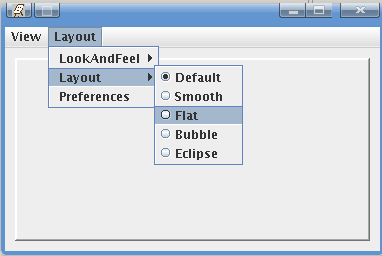
\includegraphics[scale=1]{effects/menus}
\caption{Some menus.}
\label{fig:menus}
\end{figure}

The most important class of the menu-framework is the \src{MenuPiece}. Basically a \src{MenuPiece} is a list of \src{Components} which informs observers if it changes its size. There are around 15 subclasses of \src{MenuPiece}, they allow to compose many pieces to one big piece or have more specific duties like providing the stored layouts.

An incomplete list of composing \src{MenuPiece}s contains:
\begin{description}
 \item [\src{RootMenuPiece}]: Represents a whole \src{JMenu}.
 \item [\src{SubMenuPiece}]: A wrapper around a \src{RootMenuPiece} allowing it to act like a submenu.
 \item [\src{NodeMenuPiece}]: Just a list of \src{MenuPiece}s that act like one big piece.
 \item [\src{SeparatingMenuPiece}]: A wrapper around another \src{MenuPiece} introducing separators at the top and/or bottom.
\end{description}

\classbox{Other \src{MenuPiece}s that might be interesting are:
\begin{description}
 \item [\src{BaseMenuPiece}]: A good base class for custom \src{MenuPiece}s, allows to add or remove \src{Component}s directly.
 \item [\src{FreeMenuPiece}]: A piece that does not add children by itself but has public methods which can be invoked by clients to modify the piece directly.
\end{description}
}

In the remainder of this section the more complex \src{MenuPiece}s are introduced.

\subsubsection{Themes}
\src{Common} has several themes built in, a theme tells how to paint certain components or how to react on certain events. The theme mechanism is described in more detail in chapter \ref{sec:theme}.

Clients can use a \src{CThemeMenuPiece} to quickly create a menu that changes the theme. The menu tracks any changes in the \src{ThemeMap} of the associated \src{CControl}.

\warningbox{If a \src{CThemeMenuPiece} is no longer required, then clients should call its method \src{destroy}. }

\subsubsection{LookAndFeel} \label{sec:menu:lookandfeel}
\src{Common} already supports \src{LookAndFeel}s, more about this feature can be read in chapter \ref{sec:lookandfeel}. The \src{CLookAndFeelMenuPiece} adds a menu that lists all the available \src{LookAndFeel}s and allows to exchange them.

\warningbox{If a \src{CLookAndFeelMenuPiece} is no longer required, then clients should call its method \src{destroy}. }

\infobox{Each \src{CLookAndFeelMenuPiece} will store the selection persistant, assuming that clients call \src{write} of \src{CControl} or of \src{ApplicationResourceManager}. If this behavior is not whished, then the \src{LookAndFeelMenuPiece} provides similar behavior but without the persistant storage.}

\subsubsection{Layout}
The layout is the location of all \src{dockable}s as described in chapter \ref{sec:layout}. The \src{CLayoutChoiceMenuPiece} offers users several actions to work with layouts:
\begin{description}
 \item [Save]: Saves the current layout. If the current layout has not yet a name then a dialog pops up so the user can enter a name.
 \item [Save As]: Saves the current layout but always asks the user to enter a new name for the layout.
 \item [Load]: Loads a previously saved layout, the current layout gets not stored.
 \item [Delete]: Deletes a previously saved layout.
\end{description}

\subsubsection{List of Dockables}
All closeable \src{SingleCDockable}s known to a \src{CControl} can be listed in a \linebreak \src{SingleCDockableListMenuPiece}. With this menu the user can make the \linebreak \src{dockable}s visible or invisible. The menu will update its content automatically as \src{dockable}s are added or removed from the \src{CControl}.

\subsubsection{Preferences}
\src{Common} supports preferences as described in chapter \ref{sec:preferences}. The class \linebreak \src{CPreferenceMenuPiece} adds a single item that opens a dialog with the preferences of a \src{CControl}.

\warningbox{Per default the preference system is disabled. Clients can acivate the preference system in two ways:
\begin{itemize}
 \item Call \src{setPreferenceModel} of \src{CControl} with the preferences that should be editable.
 \item Call \src{setup} of \src{CPreferenceMenuPiece} to obtain a new menu and set the default model (\src{CPreferenceModel}) in the same step.
\end{itemize}
}

